Diseñar un instrumento óptico requiere primero definir cada una de las etapas que lo componen, construirlas, alinearlas y eventualmente iterando el proceso hasta que se alcanze el objetivo del instrumental. De esta forma, es necesario medir las características de la luz antes y después de cada elemento, como ser el perfil espacial, temporal, espectral y la divergencia. 

En el Laboratorio de Electrónica Cuántica se busca construir instrumentales ópticos capaces de observar procesos biológicos y de nanoplasmónica. La mayoría de estos instrumentos, por lo tanto, son microscopios. Uno de estos instrumentos construidos en el Laboratorio se denomina SPIM (del inglés \textit{Selective/Single Plane Illumination Microscope}), que es capaz cuantificar procesos celulares tridimensionales. Este microscopio, y la implementación del LEC, está esquematizado en la figura \ref{fig:spim_lec}, basado en el trabajo de Huisken et al\cite{huisken2004}

\begin{figure}[H]
    \centering
    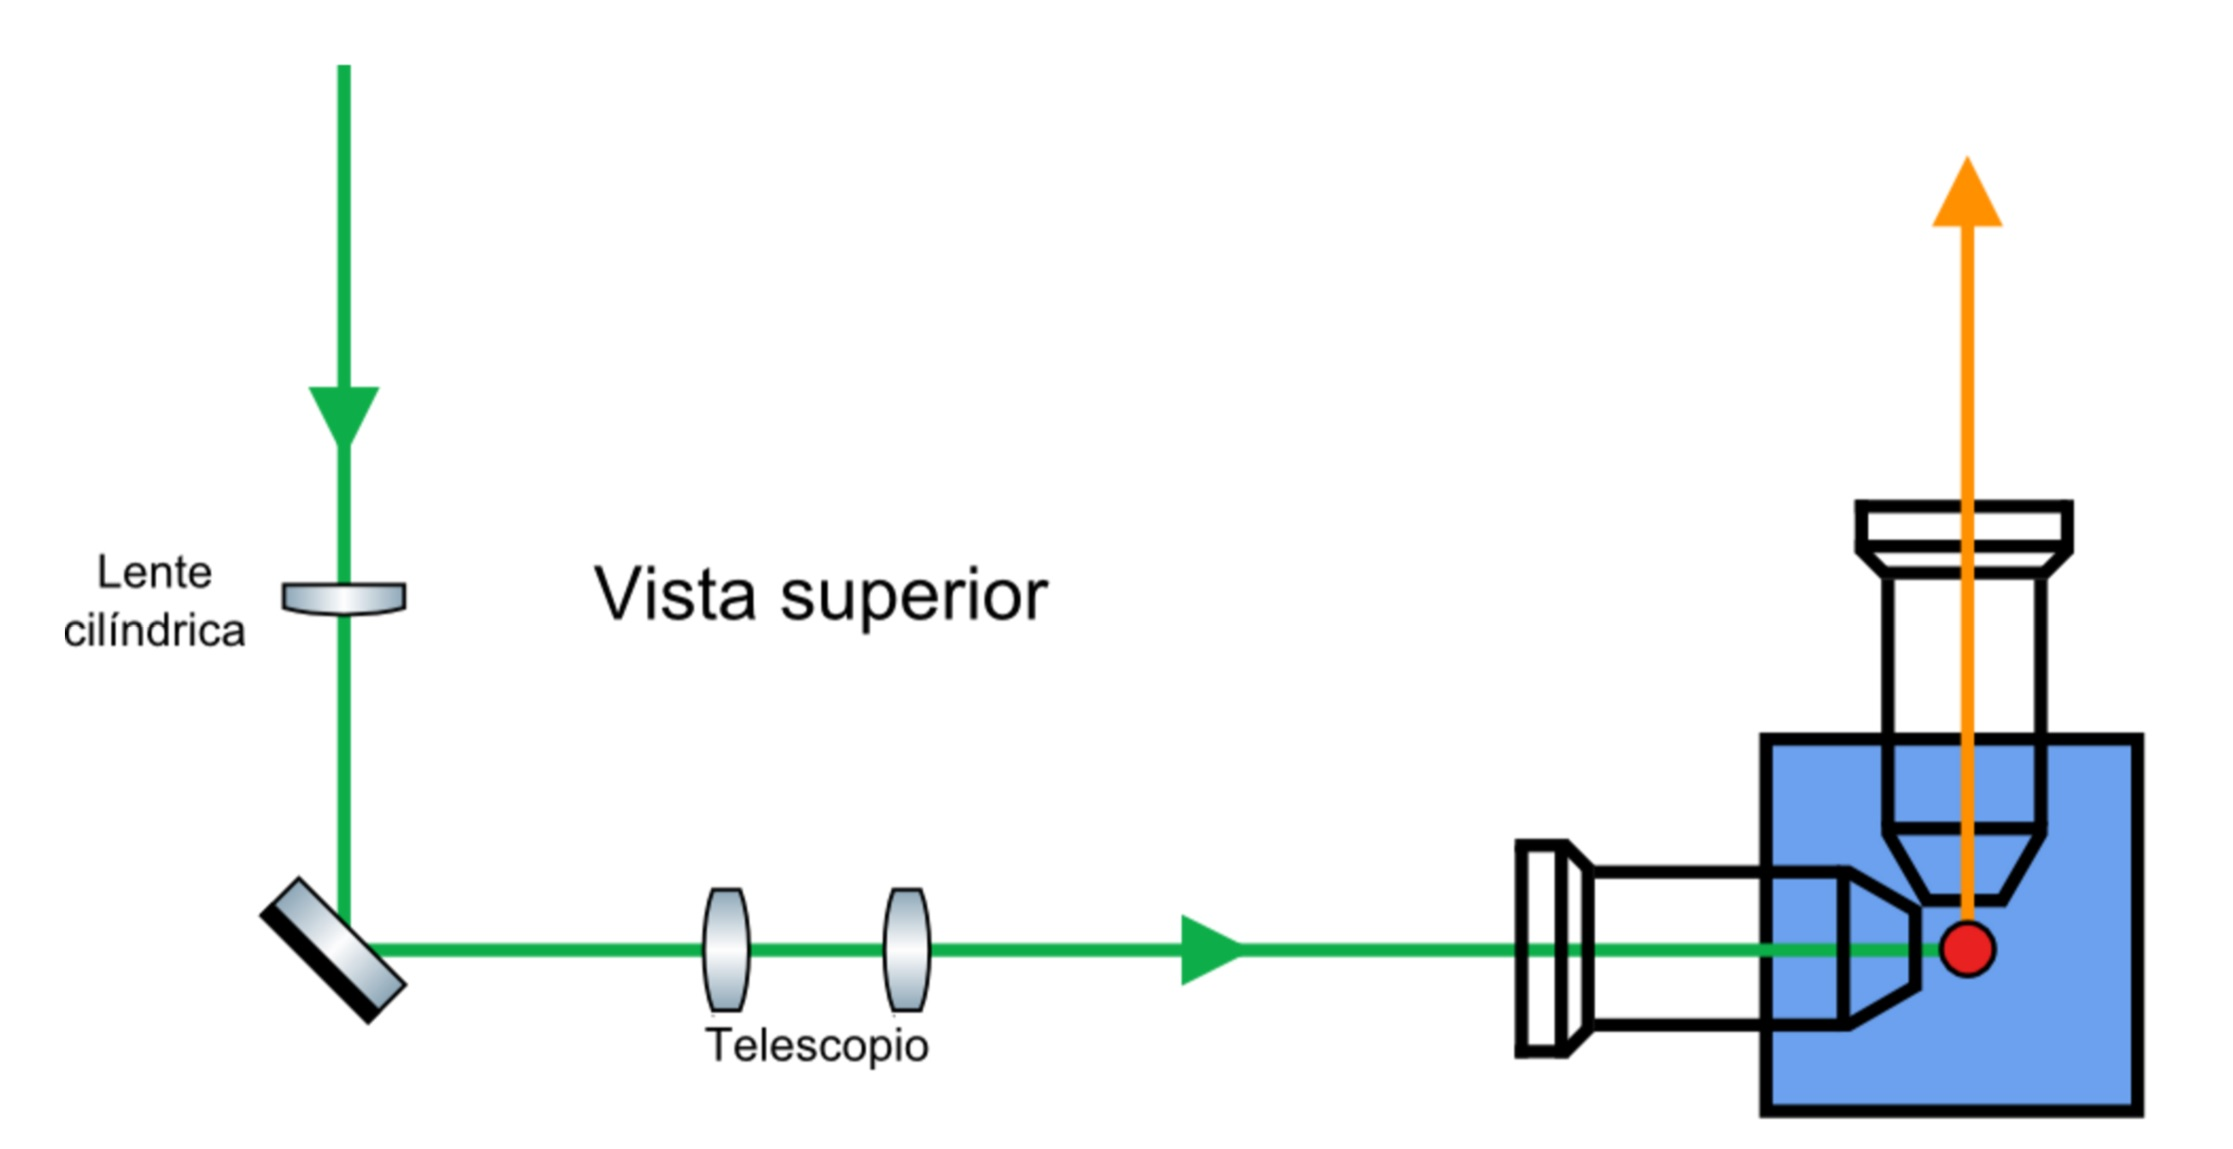
\includegraphics[width=0.6\textwidth]{fig/spim_lec}
    \caption{Esquema del microscopio SPIM del LEC, adaptado del trabajo de Huisken et al \cite{huisken2004}}
    \label{fig:spim_lec}
\end{figure}
En esta técnica se genera una hoja de luz (o \textit{lightsheet}) muy fina utilizando una lente cilíndrica. Iluminando a una muestra fluorescente con este \textit{lightsheet} y realizando una detección a 90$^{\circ}$, se logra excitar y observar a los fluoróforos de un único plano por vez. Barriendo la muestra en la dirección perpendicular del \textit{lightsheet} se colectan sucesivos planos que luego se combinan para hacer una reconstrucción tridimensional. Esto disminuye significativamente los niveles de photobleaching, es decir el blanqueado de los fluorforos, y fototoxicidad en comparación con técnicas como la microscopía confocal, en las que es necesario iluminar a la muestra completa para obtener cada plano. 

El microscopio construido en el laboratorio permite excitar fluoróforos en tres longitudes de onda (473$\,$nm, 532$\,$nm y 633$\,$nm) acopladas a una fibra óptica. Esto permite cambiar fácilmente la longitud de onda de excitación sin tener que realinear todo el sistema. A partir del análisis efectuado previamente, se concluyó que la resolución lateral del dispositivo está entre 677 y 691 nm y la resolución axial es de 5.21$\,\mu$m, con un \textit{lightsheet} de alrededor de 10$\,\mu$m de espesor. Esta resolución está en el orden de la utilizada en la referencia\cite{huisken2004} para realizar reconstrucciones tridimensionales con resolución celular del desarrollo de diversos organismos in vivo.

Uno de los objetivos del SPIM del laboratorio es poder medir la anisotropía de polarización de muestras biológicas. Esta medición consiste en iluminar las muestras con luz polarizada linealmente (en la eje mayor del lightsheet), y observar el cambio de polarización de la fluorecencia. Este proceso se encuentra esquematizado en la figura \ref{fig:fotoseleccion}, donde se produce un proceso de fotoselección de fluoroforos y posterior emisión de fluorecencia con cambios en la polarización.

\begin{figure}[H]
    \centering
    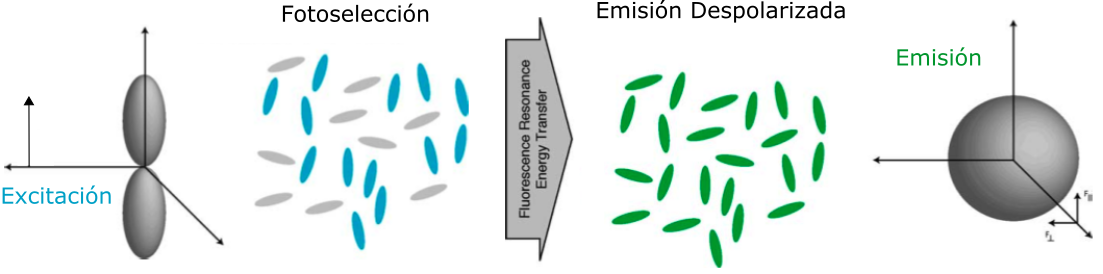
\includegraphics[width=0.8\textwidth]{fig/fotoseleccion}
    \caption{Esquema del proceso de fotoselección de flouroforos, para la posterior medición de la anisotropía}
    \label{fig:fotoseleccion}
\end{figure}

Esta magnitud permite medir procesos que cambian la estructura de los fluroforos, lo que representa un indicador para procesos biológicos de importancia para el laboratorio. De esta forma se busca poder adaptar el microscopio para poder hacer uso de estos sensores en las muestras; esto trae la necesidad de saber la polarización del haz a la salida de la fibra, para lo que también es necesario saber la polarización del haz a la entrada de dicha. Para esto, medir la polarización, se resuelve construir un instrumental para poder medirla, denominado de forma general como \emph{polarimetro}.

En la mayoría de los casos un polarímetro hace uso de polarizadores lineales, por lo que de de importancia saber como se comporta estos elementos ópticos en diferentes polarizaciones.

Si uno mide la intensidad de un haz linealmente polarizado que atravieza una lámina polarizadora lineal se observará la ley de Malus \cite{goldstein_collete}, que tiene la expresión
\begin{equation}
    I(\theta) = I_0 \cos^2(\theta)
    \label{eq:malus}
\end{equation}
donde el ángulo $\theta$ corresponde al ángulo de proyección entre el campo eléctrico incidente y el eje de la lámina. De esta forma esta expresión expresa la intensidad observada en la figura \ref{fig:polarizacion/malus}

\begin{figure}[H]
    \centering
    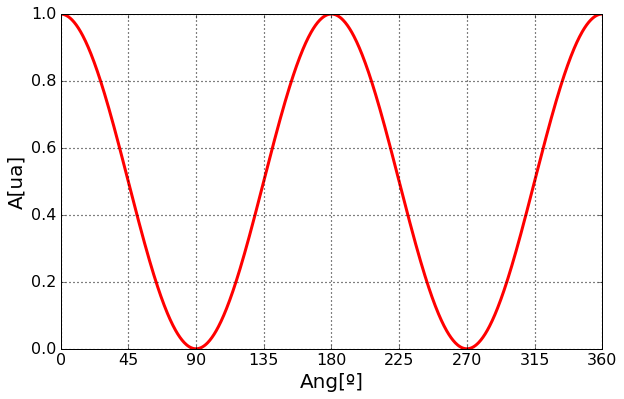
\includegraphics[width=0.38\textwidth]{fig/polarimetro/malus}
    \caption{Intensidad en función de ángulo de rotación de lámina polarizadora según la ley de Malus}
    \label{fig:polarizacion/malus}
\end{figure}

Sin embargo, si la fuente está elipticamente polarizada, uno no observará la ley de Malus si no una expresión del estilo \cite{goldstein_collett}
\begin{equation}
    I(\theta) = I_0 \cos^2(\theta) + I'_0
\end{equation}
donde la intensidad $I'_0$ agrega un offset debido a qué en hay intensidad de luz en el eje menor de la polarización. En el caso de ser circular directamente se observa una intensidad constante y si se observa polarización aleatoria no se podría hacer ningún ajuste a los datos o si el cambio de la polarización es muy rápido puede que se observe una intensidad constante.

Recordemos que el primer objetivo del polarizador es determinar el cambio de polarización que se produce al atravezar la fibra. El resultado óptimo es que a la salida de la fibra haya una polarización lineal, pero el único resultado limitante para futuras mediciones es una polarización aleatoria a la salida de la fibra. Cualquier tipo de polarización estable puede alterarse con láminas retardadoras. 

Para cuantificar la polarización a partir de la intensidad adquirida del fotodiodo se define un coeficiente de \emph{calidad de polarización lineal}, definido como
\begin{equation}
    \alpha = \frac{\max - \min}{\max + \min} = \begin{cases} 1 & \text{lineal} \\ 0 & \text{circular} \\ 0 < \alpha < 1 & \text{eliptica} \end{cases}
    \label{eq:polarizacion/alpha}
\end{equation}
que asigna un rango numérico a los tipos de polarización posible. Si la fuente tuviese una polarización aleatoria, entonces no se podría ajustar la ley de Malus o una constante correctamente.

A la hora de optimizar el tamaño del \textit{lightsheet}, y por lo tanto la resolución del microscopio, es determinante saber el tamaño del haz a la entrada delmicroscopio (en este caso de la lente cilindrica). Para poder conmensurar este parámetro del haz, se consideró la construcción de un \emph{perfilador} de haz.

Si se necesita predecir el tamaño y la divergencia del haz a la salida de un elemento óptico, es necesario conocer el haz a la entrada y la relación entre el tamaño y la divergencia de entrada y salida. Para describir esta relación, tenemos una herramienta matemática llamada matrices ABCD\cite{svelto}.

Sean dos planos perpendiculares al eje óptico, uno de entrada y otro de salida. El haz cruza el plano de entrada a una distancia $x_1$ con un ángulo $\theta_1$ respecto a la normal del plano, y lo mismo para el plano de salida con $x_2$ y $\theta_2$. La relación entre las variables se pueden escribir como una transformación matricial de la forma
\begin{equation}
{x_2 \choose \theta_2} = \begin{pmatrix} A & B \\ C & D \end{pmatrix}{x_1 \choose \theta_1} = \boldsymbol{S}  {x_1 \choose \theta_1} ,
\end{equation}

donde los números $A$,$B$,$C$, $D$ dependen solamente del objeto óptico entre el plano de entrada y salida. 

Por ejemplo, la matriz
\begin{equation}
\boldsymbol{S} = \begin{pmatrix} 1 & d \\ 0 & 1 \end{pmatrix}
\end{equation}
representa un espacio vacío de distancia $d$ entre los planos con una distancia, ya que

\[ {x_2 \choose \theta_2} = \begin{pmatrix} 1 & d \\ 0 & 1 \end{pmatrix}{x_1 \choose \theta_1} = {x_1 + d \theta_1 \choose \theta_1} \]
donde para pequeños ángulos, donde $\sen(\theta) \approx \theta$, da el resultado esperado.

Otro ejemplo, más interesante, es la representación de una lente delgada con distancia focal $f$.
\begin{equation}
\boldsymbol{S} = \begin{pmatrix} 1 & 0 \\ -\frac{1}{f} & 1 \end{pmatrix}
\end{equation}

donde en el plano de salida tenemos que
\[  {x_2 \choose \theta_2} = \begin{pmatrix} 1 & 0 \\ -\frac{1}{f} & 1 \end{pmatrix}{x_1 \choose \theta_1} = {x_1 \choose -\frac{x_1}{f} + \theta_1}\]
es decir, achica el ángulo de salida del haz dependiendo de la distancia focal y el tamaño del haz, hecho que describe correctamente el funcionamiento de una lente delgada.

Cualquier sistema óptico puede ser descripto como un matriz ABCD, que constituye un método sistemático para el trazado de rayos.

Este método puede ser fácilmente aplicado para un haz gaussiano en propagación libre. Un haz gaussiano corresponde a un haz tal que plano perpendicular a la dirección de propagación tiene una intensidad gaussiana o una campana o función de Gauss, como se ve en la figura \ref{fig:gaussian_beam_profile}

\begin{figure}[H]
\centering
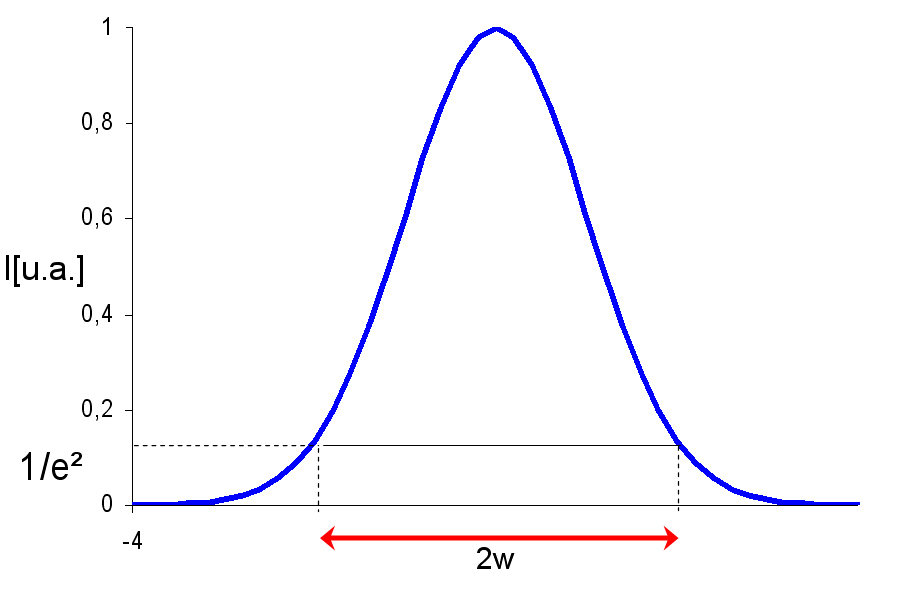
\includegraphics[width=0.35\textwidth]{fig/gaussian_beam_profile}
\caption{Perfil de intensidad de un haz gaussiano, con ancho o tamaño medio del haz parametrizado por w}
\label{fig:gaussian_beam_profile}
\end{figure}

Para estos haces se puede deducir el parámetro complejo del haz $q$ en la siguiente expresión \cite{svelto} 

\begin{equation}
    \frac{1}{q} = \frac{1}{R} - i \frac{\lambda}{\pi w^2}
    \label{eq:perfilacion/beam_parameter}
\end{equation}
donde $R$ es el radio de curvatura del haz, $lambda$ la longitud de onda y $w$ el ancho del haz. Con este parámetro y las matrices ABCD para la propagación libre ($A=D=1$, $B=z$ y $R\to\infty$, ya que no se curva el haz), se deduce que el ancho de un haz gaussiano $w$ en función del avance del haz $z$ se puede expresar como

\begin{equation}
    w(z) = w_0 \sqrt{1 + \left(\frac{\lambda z}{\pi w_0^2}\right)^2}
    \label{eq:perfilacion/gauss_divergence}
\end{equation}

donde $\lambda$ es la longitud de onda del haz y $w_0$ es la cintura del haz mínima, dada en el \emph{plano focal}. 

Este expresión se puede ver esquematizada en la figura \ref{fig:gaussian_beam_divergence}, que corresponde a un corte transversal a la propagación del haz, donde se puede apreciar la presencia del plano focal y como el haz converge y diverge de este plano

\begin{figure}[H]
\centering
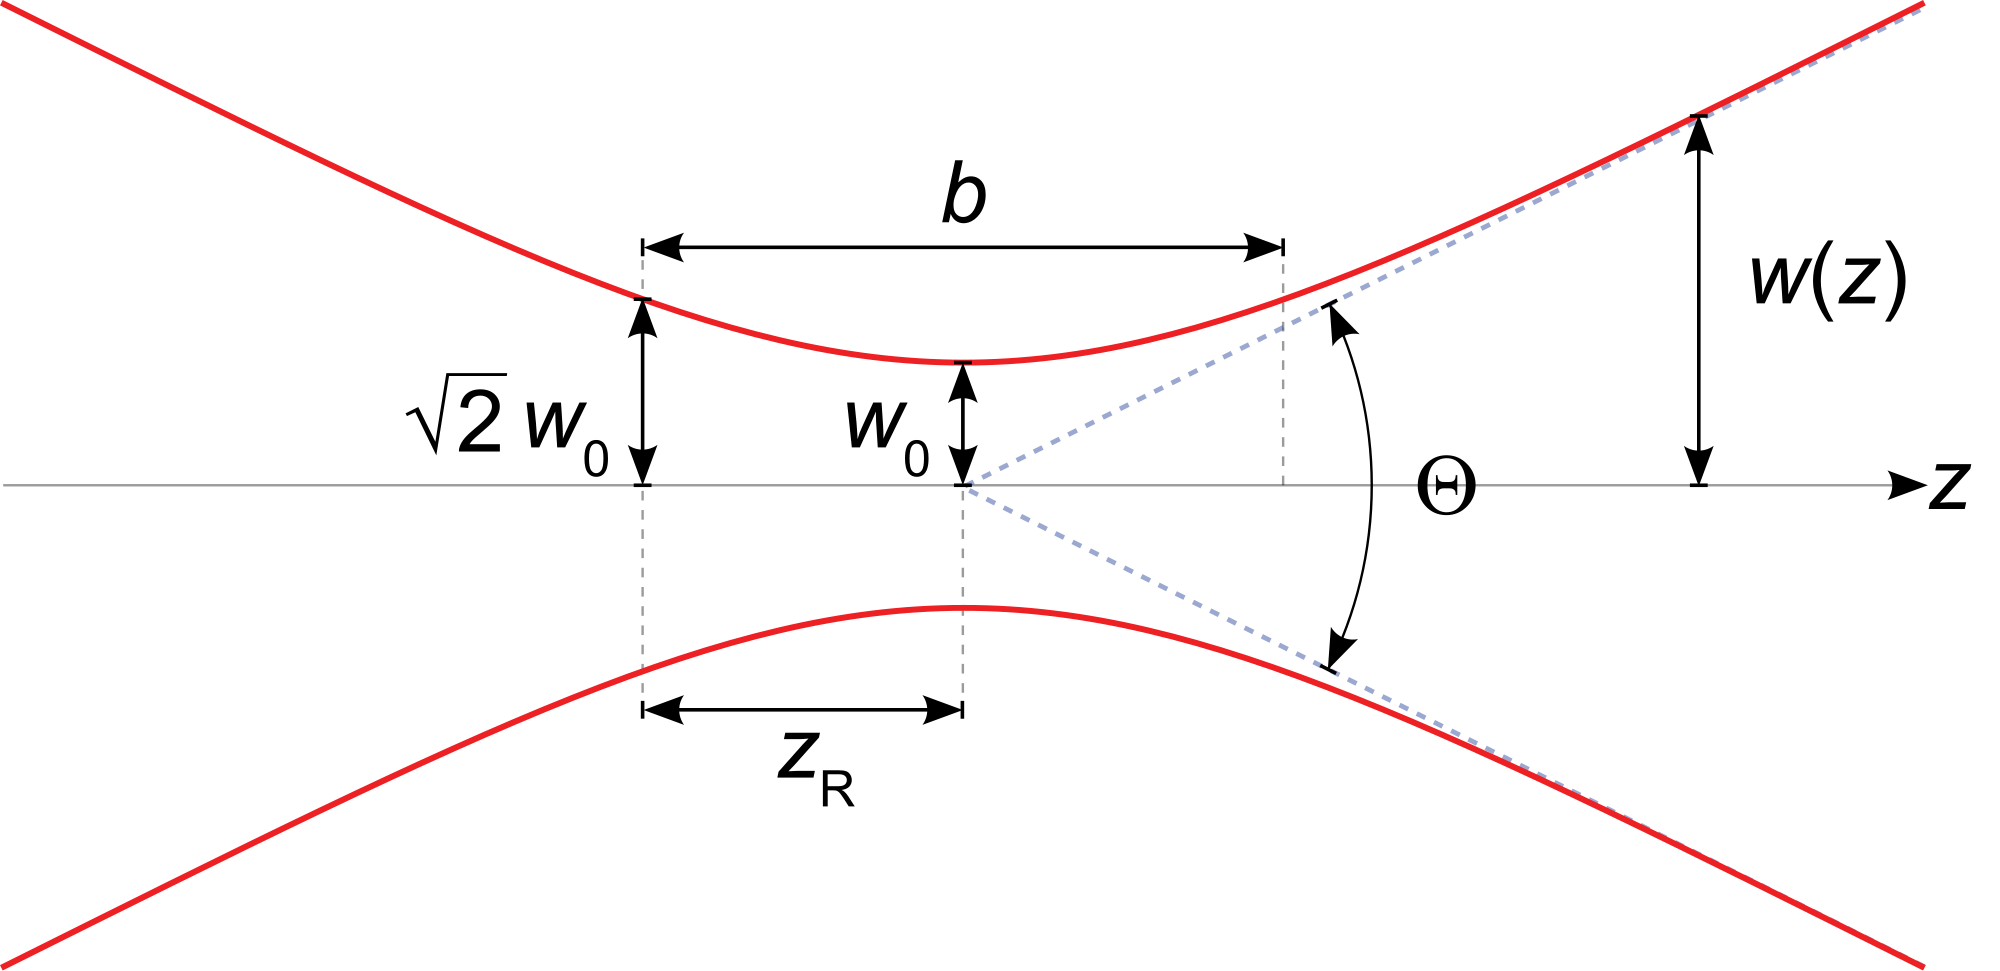
\includegraphics[width=0.35\textwidth]{fig/gaussian_beam_divergence}
\caption{Divergencia de un haz gaussiano, en este caso w$_0$ es el ancho medio mínimo del haz, en el plano focal}
\label{fig:gaussian_beam_divergence}
\end{figure}

De esta forma, el uso de matrices ABCD, especialmente para el caso guassiano, permite deducir todos los parámetros de haz y permite hacer predicciones teóricas sobre los distintos elementos ópticos utilizados en las experiencias en el laboratorio.

Para poder medir el perfil espacial y eventualmente la divergencia es necesario utilizar un perfilador de haz. Mientras tanto, para determinar la polarización de la fuente de luz se debe construir un polarimetro.

\subsection{Perfilador}

El método más usual para perfilar un haz consiste en ir obturando dicho haz y medir la potencia o intensidad del haz no obturado. El perfilador más sencillo que utiliza este concepto se puede observar en la figura \ref{fig:perfilador_basico}, que consiste en una hoja filosa (para aportar imperfecciones a la obturación) y un sensor de potencia o un sensor integrador de intensidad lumínica (como ser un fotodiodo). 

\begin{figure}[H]
\centering
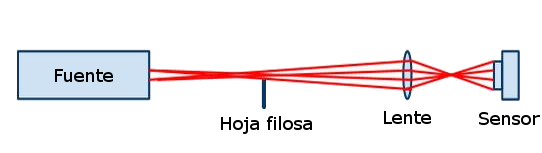
\includegraphics[width=0.35\textwidth]{fig/perfilador/esquema_basico}
\caption{Esquema de un perfilador manual}
\label{fig:perfilador/esquema_basico}
\end{figure}

Como la intensidad del haz que se mide en el fotodiodo o el sensor de potencia corresponde a la integral del haz, para un haz gaussiano vamos a observar una función error, que tiene la forma que se ve en la figura \ref{fig:err_function}

\begin{figure}[H]
\centering
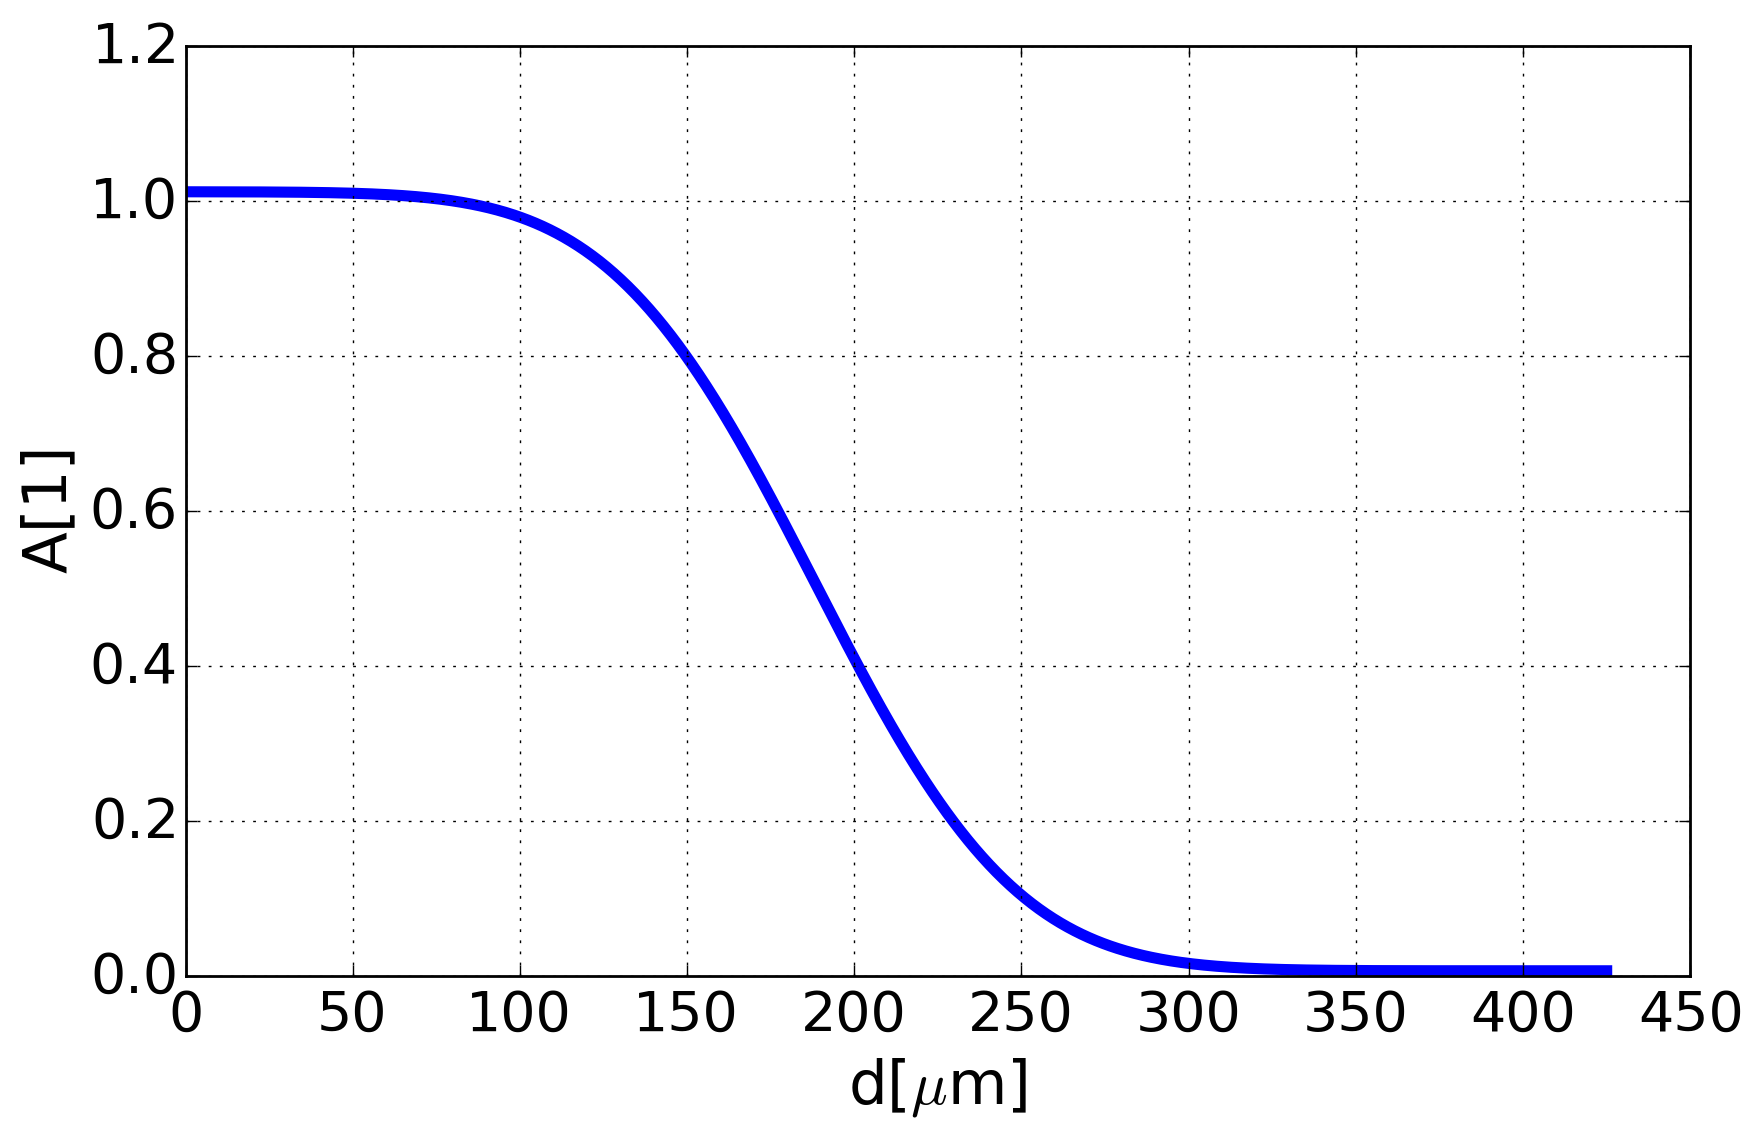
\includegraphics[width=0.4\textwidth]{fig/perfilador/err_function}
\caption{Simulación de la intensidad adquirida por un perfilador integrador en caso de un perfil gaussiano. Es un gráfico de la función error}
\label{fig:perfilador/err_function}
\end{figure}

El perfilador de Thorlabs \cite{thorlabs_profiler}, un referente comercial, consiste en un tambor giratorio con ranuras; el haz es obturado por la rendija, que define el ancho del perfil medido, la precisión la obturación y finalmente la dirección de la perfilación del haz. Después un sensor CMOS obtiene la intensidad del haz a la salida de la ranura, con su distribución espacial. 

Este perfilador es muy simple de operar, ya que no es necesario calcular ninguna derivada para observar el perfil, pero necesita un sensor CMOS con suficiente sensibilidad espacial y rango dinámico para las aplicaciones del instrumento. Esto conlleva a tener un instrumental caro solamente por el sensor, y además el equipo de Thorlabs tiene dimensiones prohibitivas para ser embebido en los setups utilizados en el laboratorio.

Mientras, el perfilador que se propone construir y caracterizar en este trabajo consiste en un tambor con rendijas (u otra estructura mecánica) que al girar obtura el haz y este es recolectado por un fotodiodo. Las rendijas o el mecanismo de obturación deben ser tal de poder obturar el haz en su totalidad y probablemente será necesario una lente para adaptar el perfilador a haces de diversos tamaños.

Otro objetivo del perfilador es lograr adquirir el perfil en tiempo real, para permitir acelerar el proceso de calibración y alineación de los setups del laboratorio. Para lograr visualizar cada medición de forma suave, la velocidad del motor y la adquisición de datos debe permitir medir perfiles y presentar en pantalla unas 24 veces por segundo, que es el límite de percepción humana donde el movimiento empieza a ser fluido.

Sin embargo, se debe considerar una medición manual del perfilador requiere entre 5 y 10 minutos, además del tiempo de colocación del instrumental, por lo que lograr medir entre 5 y 10 veces por segundo representaría una mejora subtancial al proceso de alineación y calibración.

Esta velocidad de refresco va a determinar la velocidad del tambor y la velocidad de la adquisición y acondicionamiento de los datos.

\subsection{Polarímetro}

Mientras tanto, un polarímetro es un instrumento capaz medir las propiedades de la polarización de una fuente óptica.

El modelo conceptual a utilizar se puede observar en la figura \ref{fig:polarimetro/esquema}. Este consiste en una lámina polarizadora lineal que puede rotar en un coaxial o perpendicular al plano de polarización, y al hacer este movimiento va cambiando el plano de polarización. En cada nuevo plano se transforma la luz transferida en señal eléctrica con un sensor integrador como un sensor de potencia o un fotodiodio. 

\begin{figure}[H]
    \centering
    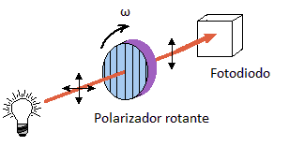
\includegraphics[width=0.45\textwidth]{fig/polarimetro/esquema}
    \caption{Esquema conceptual del polarímetro, donde se observa la fuente de luz, con alguna polarización a determinar, la lámina rotante polarizadora y el sensor de luz integrador, en este caso un fotodiodo}
    \label{fig:polarimetro/esquema}
\end{figure}

Como el fotodiodo mide la intensidad lumínica, la señal que se va adquirir sigue la ley de Malus, ecuación \ref{eq:polarizacion/malus}, si es una polarización lineal, o una intensidad parecida más offset. De esta forma se puede usar el coeficient $\alpha$ para cuantificar la polarización a partir de esta señal.

Respecto a la velocidad de adquisición del instrumental, nuevamente se requiere adquirir en tiempo real, para poder observar la polarización mientras se altera láminas retardadoras y la alineación de algunos elementos ópticos. Dado que una medición manual tarda entre 5 a 10 minutos, con lograr entre 5 y 10 mediciones por minuto se acortaría considerablemente los tiempos de trabajo.
